\section{Rundkurs ohne Hindernisse}
	Bei dieser Aufgabe muss das Auto einen bekannten Rundkurs im Flur des Instituts in 	m�glichst kurzer Zeit bew�ltigen. 

  \subsection{Grundidee}
    Der Rundkurs besteht aus Geraden, an deren Ende sich jeweils eine Kurve befindet. Demnach existieren in diesem System zwei Hauptzust�nde: \glqq Fahrzeug auf der Geraden\grqq ~oder \grqq Fahrzeug in Kurve\grqq. Die Modellierung des Ganzen als Zustandsautomat erscheint also sinnvoll.
    
\begin{figure}[htbp]
    \centering
    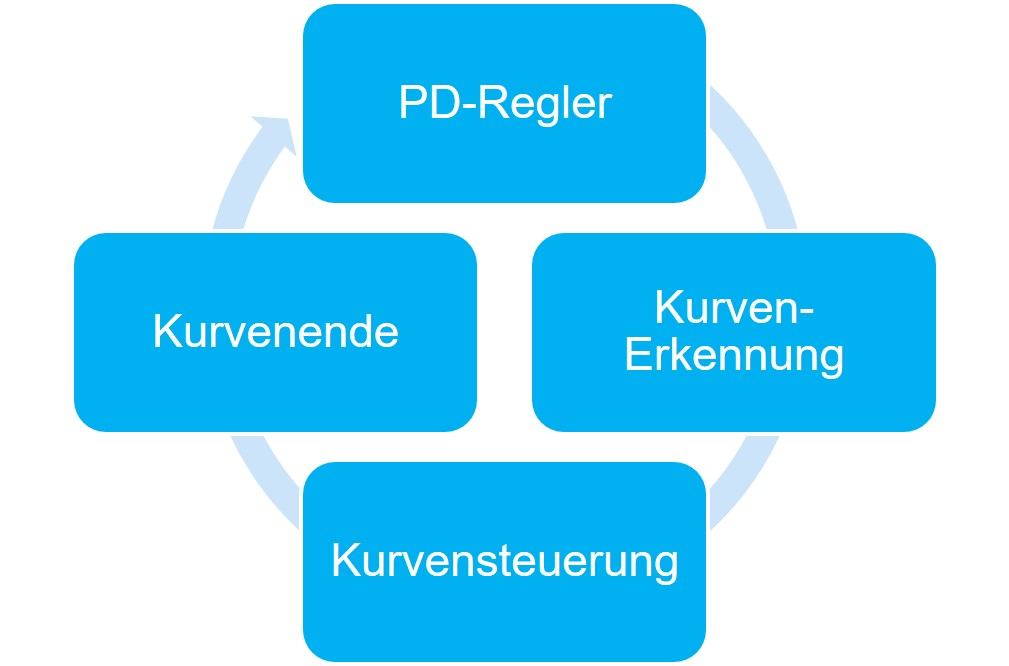
\includegraphics[width=0.5\textwidth]{images/rndkOhneZustandsdiag.jpg}
    \caption {Zustandsdiagramm}
    \label{fig: Zustandsdiagramm}
\end{figure}

  \subsection{Regelung der Fahrt auf den Geraden}
	Jede Gerade hat den Vorteil, dass sie durch eine Wand begrenzt ist, an welcher sich das Fahrzeug orientieren kann. Der aktuelle Abstand zur Wand kann n�mlich n�herungsweise mit dem Ultraschall-Sensor, der auf der linken Seite des Autos montiert ist, bestimmt 		werden. Mit Hilfe eines PD-Reglers wird sichergestellt, dass sich das Auto parallel zur 	Wand fortbewegt.
	\\
	Die dazu ben�tigten Parameter wurden bei Testfahrten empirisch ermittelt. Au�erdem 		werden die Messwerte des Ultraschall-Sensors gegl�ttet, um nerv�se Lenkbewegungen zu 		vermeiden, indem aus den letzten 10 Messwerten ein Mittelwert gebildet wird.      

  \subsection{Steuerung der Fahrt in den Kurven}
  	Zu Beginn wurde auch hier versucht, das Problem mittels einer Regelung zu l�sen. Mit der Zeit sollte sich jedoch herausstellen, dass eine simple Steuerung bessere Ergebnisse 	erzielt. In der Kurve wird also einfach ein fester Lenkwinkel eingestellt, der w�hrend 		der gesamten Kurvenfahrt konstant bleibt.
  	
  \subsection{Kurvenerkennung}
  	Die Kurvenerkennung entspricht im Zustandsautomaten dem �bergang von der Geraden hin zur	Kurve. Wie erkennt man also eine Kurve? Verl�sst man sich ausschlie�lich auf den 		Ultraschall-Sensor, kann man eine Kurve erst detektieren, wenn sich links des Fahrzeugs 	keine Wand mehr befindet. Dann befindet sich das Auto allerdings schon mitten im 			Kurvenbereich und eine vern�nftige Linie kann keinesfalls mehr erreicht werden.

\begin{figure}[htbp]
    \centering
    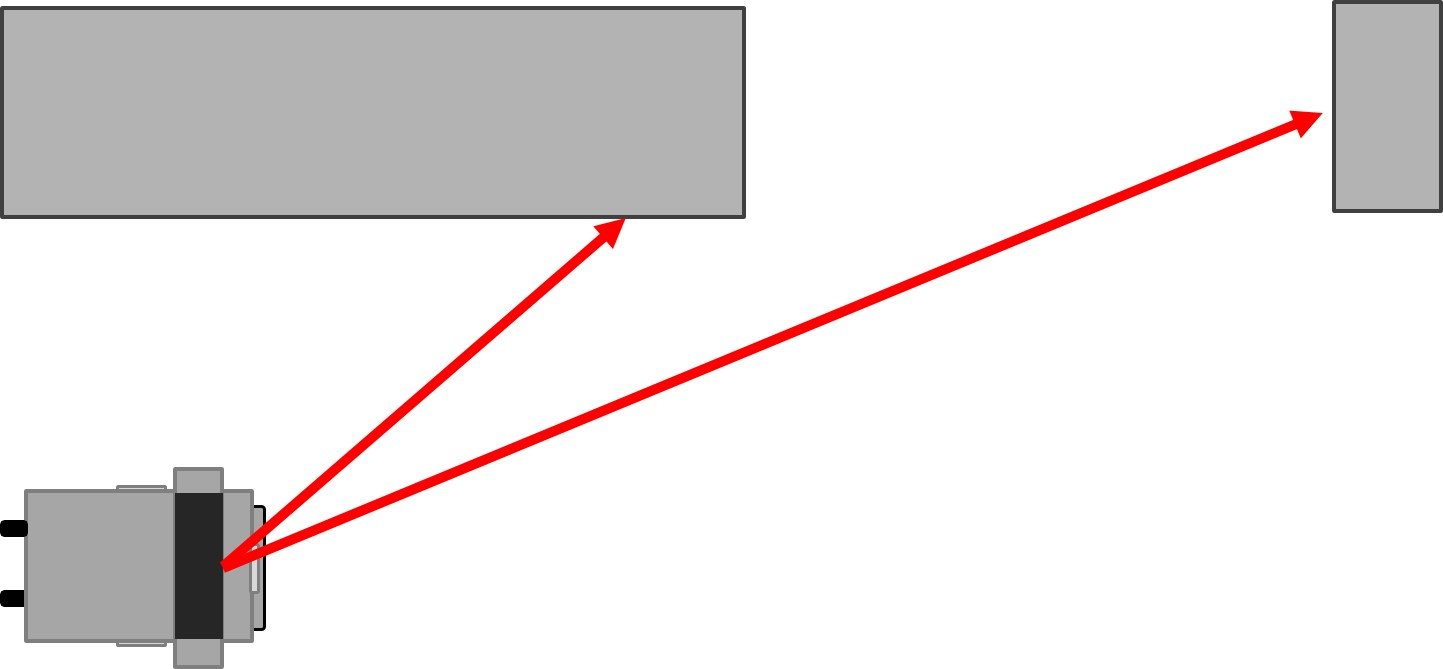
\includegraphics[width=0.5\textwidth]{images/rndkOhneKurvenerkennung.jpg}
    \caption {Kurvenerkennung}
    \label{fig: Kurvenerkennung}
\end{figure}

	An dieser Stelle kommt die Kinect-Kamera ins Spiel. Durch sie ist es m�glich, bereits 	deutlich vor einer anstehenden Kurve selbige zu erkennen. Somit wird es �berhaupt erst 		m�glich eine optimale Kurvenlinie zu fahren.
	\\
	Auf diesem Rundkurs zeichnet sich eine Kurve dadurch aus, dass am Kurvenbeginn die Wand abrupt endet. Die gemessenen Distanzen im von der Kinect generierten Laserscan steigen an dieser Stelle also sprunghaft an, was detektiert werden kann.  
  
  \subsection{Kurvenende}	
  	Der vorgegebene Rundkurs enth�lt ausschlie�lich 90�-Kurven. Am Kurvenausgang ist demnach der Gierwinkel des Fahrzeugs etwa 90� gr��er als am Kurveneingang. Steigt der Gierwinkel also �ber einen gewissen Schwellwert, �bernimmt der PD-Regler wieder die Kontrolle.
  	
  \subsection{Probleme}
   \subsubsection{Kurvenerkennung am Kurvenausgang}
  Am Kurvenausgang, wenn gerade wieder auf den PD-Regler umgeschaltet wurde, befindet sich die linke Wand nicht unbedingt im Sichtfeld der Kinect. Dadurch kommt die weiter oben beschriebene Kurvenerkennung aus dem Tritt. Es kommt zu einem False-Positive: Eine Kurve wird in der Punktmenge des Laserscans erkannt, die gar nicht existiert. In Folge dessen lenkt das Auto direkt in die Wand.
  \\
  Durch Einf�hrung einer Totzeit kann dieses Problem gel�st werden. Nachdem eine Kurve beendet wurde, muss erst eine gewisse Zeitspanne vergehen, bis die Kurvenerkennung reaktiviert wird. Dann ist die Wand schon wieder im Sichtfeld und die Kurvenerkennung arbeitet somit wieder korrekt.
  
   \subsubsection{Glaserkennung}
  Auf dem Rundkurs befindet sich ein Besprechungsraum mit mehreren Glasscheiben. Durch diese schaut die Kinect einfach durch. In dem daraus resultierenden Laserscan wird auch hier wieder eine Kurve erkannt werden.
  \\
  In einer Eigenschaft unterscheiden sich allerdings Glasscheiben von echten Kurven: Die breiteste Glasscheibe misst etwa 80cm in der Breite, der schmalste Flur 160cm. F�r den Fall, dass eine Ecke erkannt wird, wird in einem Bereich nach der Ecke �berpr�ft, ob sich dort Objekte befinden. Durch geeignete Wahl dieses Bereichs kann zwischen \glqq echten\grqq ~und \glqq falschen\grqq ~Kurven unterschieden werden.

\begin{figure}[htbp]
    \centering
    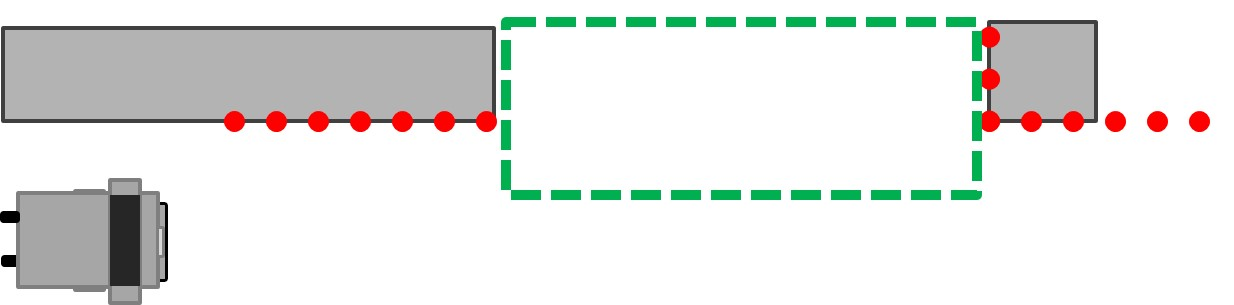
\includegraphics[width=0.5\textwidth]{images/rndkOhneKeinGlas.jpg}
    \caption {Glaserkennung an Kurven}
    \label{fig: Glaserkennung an Kurven}
\end{figure}

\begin{figure}[htbp]
    \centering
    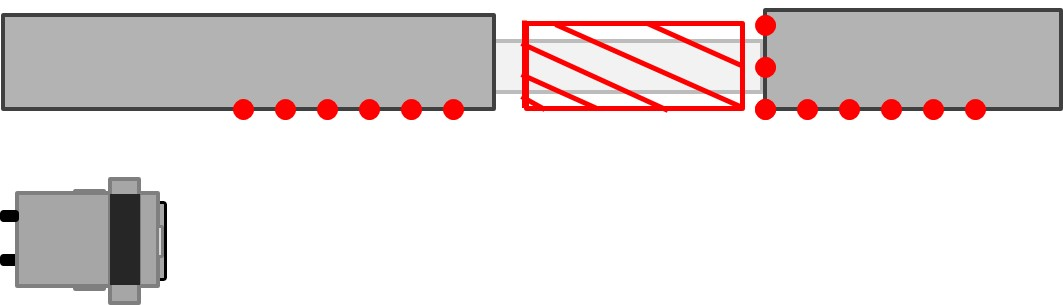
\includegraphics[width=0.5\textwidth]{images/rndkOhneGlas.jpg}
    \caption {Glaserkennung an Glasscheiben}
    \label{fig: Glaserkennung an Glasscheiben}
\end{figure}

  Dar�ber hinaus ist die Glaserkennung nicht nur f�r Glasscheiben n�tzlich. Wegen wahrscheinlich von LED-Lampen verursachten St�rungen treten sporadisch L�cken in der Wand auf. Da sich diese L�cken hinsichtlich der Glaserkennung allerdings exakt gleich verhalten, wurde dieses Problem hiermit bereits adressiert.
  
  \subsubsection{Begrenztes Sichtfeld der Kinect}
  Der Winkel des Sichtfeldes der Kinect ist stark begrenzt. In Folge dessen kann es passieren, dass eine Ecke, der man zu nahe kommt, aus dem sichtbaren Bereich verschwindet. Die Position der Ecke muss also gespeichert werden solange die Kinect sie noch sieht. Anschlie�end kann mit Hilfe der Odometrie der korrekte Einlenkzeitpunkt bestimmt werden.
  
\begin{figure}[htbp]
    \centering
    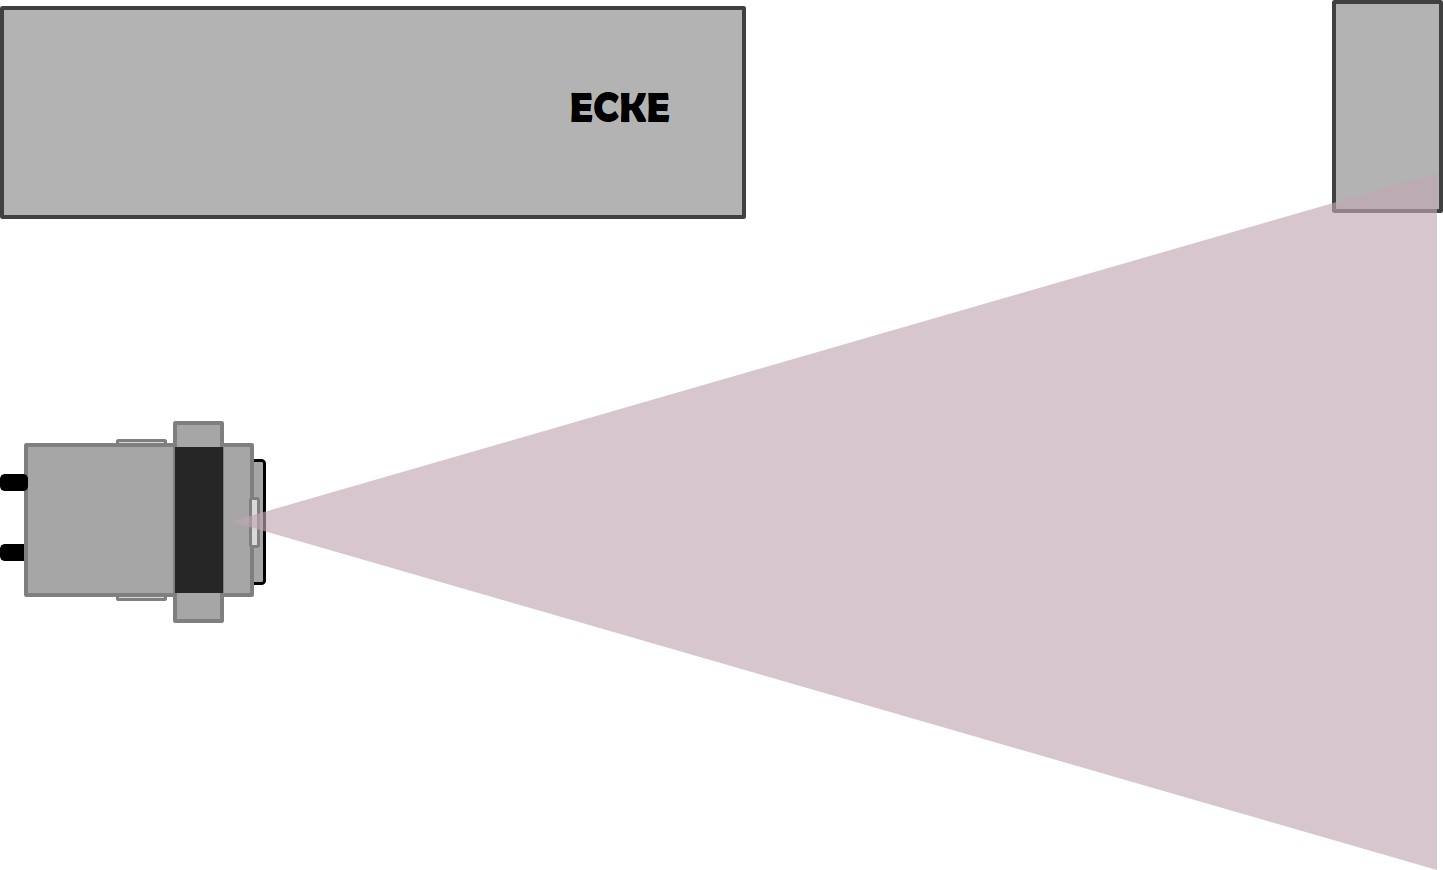
\includegraphics[width=0.5\textwidth]{images/rndkOhneSichtfeld.jpg}
    \caption {Sichtfeld der Kinect}
    \label{fig: Sichtfeld der Kinect}
\end{figure}

  \subsubsection{Entkopplung von Geraden- und Kurvengeschwindigkeit}
  Bei h�heren Geschwindigkeiten kann es sinnvoll sein, in den Kurven langsamer zu fahren als auf den Geraden. Ein normales Auto w�rde dazu sicherlich vor den Kurven abbremsen, bei diesem Modell ist es ausreichend kurz vor den Kurven den Motor abzuschalten.
\\    
  Um die Strecke zu bestimmen, wie weit das Fahrzeug vor der Kurve vom Gas gehen muss, wurden folgende Berechnungen durchgef�hrt.